\documentclass[11pt,a4paper]{article}

% Packages
\usepackage[utf8]{inputenc}
\usepackage[spanish, es-tabla]{babel}
\usepackage{caption}
\usepackage{listings}
\usepackage{adjustbox}
\usepackage{enumitem}
\usepackage{hyperref}
\usepackage{boldline}
\usepackage{amsmath}
\usepackage{amssymb, amsmath}
\usepackage[margin=1in]{geometry}
\usepackage{xcolor}
\usepackage{xlop}
\usepackage{soul}
\usepackage[ruled,vlined,linesnumbered]{algorithm2e}
\usepackage{amsthm} %Paquete para la terminología matemática
\usepackage[ruled,vlined,linesnumbered]{algorithm2e}
\usepackage{subfigure}
\usepackage{listings}
\usepackage{color}

\definecolor{dkgreen}{rgb}{0,0.6,0}
\definecolor{gray}{rgb}{0.5,0.5,0.5}
\definecolor{mauve}{rgb}{0.58,0,0.82}

\lstset{frame=tb,
  language=Python,
  aboveskip=3mm,
  belowskip=3mm,
  numbers=left,
  stepnumber=1,
  showstringspaces=false,
  columns=flexible,
  basicstyle={\small\ttfamily},
  numberstyle=\tiny\color{gray},
  keywordstyle=\color{blue},
  commentstyle=\color{dkgreen},
  stringstyle=\color{mauve},
  breaklines=true,
  breakatwhitespace=true,
  tabsize=3
}
%Entorno de la librería matemática (Macros para que no salga en inglés).
\newtheorem{theorem}{Teorema}[section]
\newtheorem{corollary}{Corolario}[theorem]
\theoremstyle{definition}
\newtheorem{definition}{Definición}[section]

% Meta
% Custom
\providecommand{\abs}[1]{\lvert#1\rvert}
\setlength\parindent{0pt}
\definecolor{Light}{gray}{.90}
\newcommand\ddfrac[2]{\frac{\displaystyle #1}{\displaystyle #2}}
\newcommand\tab[1][1cm]{\hspace*{#1}}

\begin{document}
\begin{titlepage}
  \centering
 
\includegraphics[width=0.15\textwidth]{./images/exp.jpg}\par\vspace{1cm}
  {\scshape\LARGE Universidad de Granada  \par}
  \vspace{1cm}
  {\scshape Proyecto Final\par}
  \vspace{1.5cm}
  {\huge\bfseries  Clasificación de radiografías torácicas para detección de COVID-19\par}
  \vspace{2cm}
  {\Large\itshape Alberto Luque Infante\\David Villar Martos\par}
  \vfill
  Quinto curso del Doble Grado de Ingeniería Informática y Matemáticas:\par
  Visión por Computador

  \vfill

% Bottom of the page
  {\large \today\par}
\end{titlepage}

\tableofcontents
\newpage
\section{Descripción del proyecto}

El proyecto consiste en abordar el problema de clasificación de radiografías torácicas con la intención de poder detectar casos positivos de COVID-19.\\

Partiendo de un modelo de red convolucional preentrenado con la base de datos ImageNet, utilizarlo como base para encontrar el mejor modelo que nos permita llevar a cabo esta tarea.\\

En la base de datos escogida se utilizan imágenes clasificadas en tres clases distintas: radiografías de pulmones sanos (NORMAL), radiografías de pulmones en casos positivos de COVID-19 (COVID) y radiografías de pulmones afectados con neumonía vírica (Viral Pneumonia).\\

Por tanto, nuestro problema de clasificación va a consistir en implementar un modelo que nos permita clasificar estas imágenes en las tres clases.\\

Primero haremos un análisis previo del problema para poder enfocarlo correctamente. A continuación comenzaremos con la lectura y preprocesamiento de los datos, conformando los conjuntos de train y test.\\

Hemos elegido como modelo inicial preentrenado con ImageNet el modelo DenseNet121. Partiendo de una primera versión muy básica poco a poco le iremos añadiendo mejoras hasta encontrar el modelo más óptimo.\\

Posteriormente, utilizaremos otros modelos conocidos preentrenados también en ImageNet para poder compararlos entre sí.\\

Finalmente, vamos realizar un análisis pormenorizado de los resultados obtenidos, visualizando los mapas de activación y mapas de calor con el objetivo de detectar qué zonas de las imágenes de entrada son más discriminativas de cara a realizar la clasificación. De esta forma podremos entender un poco mejor el modelo y extraer conclusiones que puedan ayudar también al campo de la medicina.\\

Por último, comentaremos algunas propuestas o aspectos que se podrían mejorar en un futuro en base a la experiencia obtenida.\\


\newpage

\section{Análisis previo del problema}

AQUI PODRIAN IR COSAS DE LAS QUE TE PASO TU AMIGO DE MEDICINA

\section{Base de Datos elegida para el problema}
\subsection{Información de la Base de Datos}
La base de datos elegida para el proyecto se encuentra en Kaggle :

https://www.kaggle.com/tawsifurrahman/covid19-radiography-database.\\

La base de datos, en su actualización del 5 de enero de 2021 (versión 3), contiene un total de 1200 imágenes de la clase COVID, 1341 imagenes de la clase NORMAL y 1345 imágenes de la clase Viral Pneumonia.\\

El conjunto de imágenes del dataset proceden de distintas fuentes. Las imágenes de la clase COVID proceden, entre otras fuentes, de un colegio médico alemán y del SIRM (Italian Society of Medical and Interventional Radiology).\\

Para las clases NORMAL y Viral Pneumonia también se han utilizado imágenes de distintas bases de datos públicas, algunas de ellas pertenecientes al ESR (European Society of Radiology).\\

\subsection{Lectura de la Base de Datos}

Para que las clases estén equilibradas vamos a tomar el mismo número de imágenes por clase, 1200, luego tendremos un total de 3600 imágenes.\\

Para leer las imágenes, creamos un vector de etiquetas con las 1200 etiquetas para cada clase y utilizamos la función implementada \textit{leerImagenes}.\\

Leemos las imágenes de cada clase interpolando para que tengan un tamaño de (224,224), que es el tamaño que tienen las imágenes de ImageNet.\\
\begin{lstlisting}
def leerImagenes(clases, num_imgs, path):
  
  imgs_covid = np.array([img_to_array(load_img(path + "/" + clases[i] + "/" + clases[i] + " (" + str(i+1) + ").png",
                                                target_size = (224, 224), interpolation="bilinear")) for i in range(0,num_imgs)])
  imgs_normal = np.array([img_to_array(load_img(path + "/" + clases[i] + "/" + clases[i] + " (" + str(i-num_imgs+1) + ").png",
                                                target_size = (224, 224), interpolation="bilinear")) for i in range(num_imgs,2*num_imgs)])
  imgs_viral = np.array([img_to_array(load_img(path + "/" + clases[i] + "/" + clases[i] + " (" + str(i-2*num_imgs+1) + ").png", 
                                                target_size = (224, 224), interpolation="bilinear")) for i in range(2*num_imgs,3*num_imgs)])

  return imgs_covid, imgs_normal, imgs_viral
\end{lstlisting}

Un ejemplo de una imagen de cada clase es el siguiente:

\begin{figure}[h]
  \centering
  \begin{minipage}[b]{0.25\textwidth}
    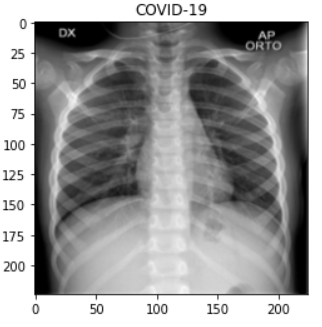
\includegraphics[scale=0.65]{./images/ejemploCOVID}
	\caption{Imagen de la clase COVID}
  \end{minipage}
  \hfill
  \begin{minipage}[b]{0.25\textwidth}
    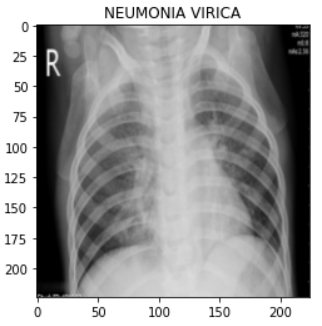
\includegraphics[scale=0.65]{./images/ejemploNEUMONIAVIRICA}
	\caption{Imagen de la clase Viral Pneumonia}
  \end{minipage}
    \hfill
    \begin{minipage}[b]{0.25\textwidth}
    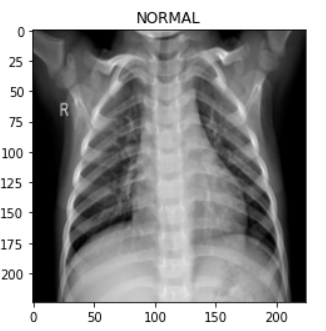
\includegraphics[scale=0.65]{./images/ejemploNORMAL}
	\caption{Imagen de la clase NORMAL}
  \end{minipage}
\end{figure}


\subsection{Creación de los conjuntos de train y test}

Primero creamos un vector agrupando las imágenes de las tres clases y cambiamos las etiquetas por números enteros, asignando el valor 0 a la clase COVID, el 1 a la clase NORMAL y el 2 a la clase Viral Pneumonia.\\

A continuación, usando la función \textit{to\_categorical} obtenemos una representación binaria de las clases (la clase 0 pasa a ser [1,0,0], la 1 es [0,1,0] y la 2 es [0,0,1]).\\

Después de hacer una permutación de las imágenes, dividimos en proporción 80\%-20\% para obtener los conjuntos de entrenamiento y de test, obteniendo 2880 imágenes para entrenar y 720 para test.



\section{Implementación de los modelos}

\subsection{DenseNet121}

DenseNet121 es el modelo que hemos elegido para empezar. En las primeras versiones vamos a utilizar el modelo, con los pesos de ImageNet, solo como extractor de características, a partir del cuál añadiremos modificaciones. Finalmente, haremos un ajuste fino del modelo donde sí moveremos los pesos.

\subsubsection{Version 0: Extractor de características inicial, sin entrenamiento}

Primero vamos a utilizar el modelo DenseNet121 preentrenado con IMAGENET sin entrenar ningún peso. Partiendo de las características extraídas, simplemente vamos a añadir la capa softmax y comprobaremos que los resultados no son para nada buenos, pues todavía no hemos entrenado nuevos pesos, no estamos adaptando la red a nuestros datos en absoluto.

Extraemos las características:

\begin{lstlisting}
#Definicion inicial de nuestro modelo preentrenado en imagenet.
#Para usarlo como extractor de caracteristicas simple

#Vamos a cargar el modelo antes del ultimo pooling, para usarlo como extractor de caracteristicas
feat_extractor = DenseNet121(include_top=False, weights='imagenet', pooling='avg')
feat_extractor.trainable = False

#Una vez tenemos el modelo, vamos a compilarlo usando un optimizador y una funcion de perdida
opt = SGD(lr=0.01, decay= 1e-6, momentum=0.9, nesterov=True)

feat_extractor.compile(optimizer=opt, loss="categorical_crossentropy", metrics=["acc"])

#Con esto tenemos el modelo de densenet hasta que nos deja los datos en forma de vector unidimensional
#de dimension 1024
feat_extractor = keras.Model(inputs=feat_extractor.inputs, outputs= feat_extractor.layers[-1].output)

feat_extractor.compile(optimizer=opt, loss="categorical_crossentropy", metrics=["acc"])

# Extraer las caracteristicas de las imagenes con el modelo anterior.
car_train = feat_extractor.predict(x_train, verbose=1)
car_test = feat_extractor.predict(x_test, verbose=1)
\end{lstlisting}

Una vez tenemos las características, añadimos la capa softmax y hacemos las predicciones.

\begin{lstlisting}
inputs = keras.layers.Input(shape=[1024])
outputs = keras.layers.Dense(units=3, activation="softmax")(inputs)


dense_model = keras.Model(inputs=inputs, outputs=outputs)
opt = SGD(lr=0.01, decay= 1e-6, momentum=0.9, nesterov=True)
dense_model.compile(optimizer=opt, loss="categorical_crossentropy", metrics=["acc"])

#Clasificamos
y_preds = dense_model.predict(car_test, verbose=True)

print("La accuracy del modelo es: " + str(calcularAccuracy(y_test, y_preds)))

y_test_conf = np.argmax(y_test, axis=1)
y_preds = np.argmax(y_preds, axis=1)
print("La matriz de confusion de las predicciones ha sido: \n", confusion_matrix(y_test_conf, y_preds))
\end{lstlisting}

FALTAN RESULTADOS CUANDO EJECUTEMOS CON TODAS LAS IMGS

\subsubsection{Version 1: Extractor de características inicial, entrenando la capa de salida}

Ahora vamos a reentrenar sólo la capa de salida, sin ningún tratamiento adicional. La única diferencia respecto a la versión anterior es que sí que entrenamos la última capa:

\begin{lstlisting}
hist = dense_model.fit(car_train, y_train, batch_size=32, epochs=20, validation_split=0.1)
\end{lstlisting}

RESULTADOS...........


\subsubsection{Version 2: Data augmentation, más capas densas}

Seguimos empleando la red preentrenada como extractor de características pero se realiza un preprocesado más exhaustivo de imágenes, con image augmentation y normalización, además de hacer un modelo denso de mayor profundidad.\\

Además de hacer una normalización de las imágenes, para que tengan media cero y varianza 1, hemos detectado que hay imágenes que salen muy blancas y otras muy oscuras, luego debemos conseguir invarianza frente al brillo (añadiendo el parámetro brightness).\\

En cuanto al data augmentation, los pulmones en las radiografías salen siempre verticales, por lo que no tiene mucho sentido añadir rotaciones pero sí flips horizontales. Los zooms de ampliación también pueden ser interesantes, puesto que las imágenes tienen siempre los pulmones en la zona central, y podemos evitar posibles fuentes de ruido de letras que tienen algunas de las imágenes en las zonas laterales, que se perderán haciendo zoom.\\

Para aplicar todo esto, creamos un objeto de la clase ImageDataGenerator:

\begin{lstlisting}
#Image data generators

train_generator = ImageDataGenerator(featurewise_center = True,
                             featurewise_std_normalization = True,
                             validation_split=0.1,
                             horizontal_flip=True,
                             brightness_range=[0.8,1.25],
                             zoom_range=[1,1.2])
train_generator.fit(x_train)

test_generator = ImageDataGenerator(featurewise_center = True,
                             featurewise_std_normalization = True)

test_generator.fit(x_train)

it = train_generator.flow(x_train, batch_size=1)
\end{lstlisting}

Añadimos también alguna capa densa más para ganar profundidad:

\begin{lstlisting}
inputs = keras.layers.Input(shape=[1024])
layer1 = keras.layers.Dense(units=500, activation="relu")(inputs)
layer2 = keras.layers.Dense(units=200, activation="relu")(layer1)
outputs = keras.layers.Dense(units=3, activation="softmax")(layer2)
\end{lstlisting}


RESULTADOS..........


En esta última versión puede ser que tengamos un poco de overfitting puesto que el validation loss no decrece al mismo ritmo que el training loss. Regularizamos añadiendo una capa de Dropout.

\begin{lstlisting}
inputs = keras.layers.Input(shape=[1024])
layer1 = keras.layers.Dense(units=500, activation="relu")(inputs)
layer2 = keras.layers.Dropout(0.5)(layer1)
layer3 = keras.layers.Dense(units=200, activation="relu")(layer2)
outputs = keras.layers.Dense(units=3, activation="softmax")(layer3)
\end{lstlisting}

RESULTADOS................


\subsubsection{Version 3: Fine tunning}

Vamos a probar ahora a hacer un ajuste fino de la red completa, tomando como pesos iniciales los de imagenet. Ahora ya no solo vamos a utilizar DenseNet como extractor de características, sino que, en vez de estar la red congelada, vamos a ir moviendo sus pesos con el entrenamiento.

\subsection{ResNet50}

\subsection{VGG19}

\subsection{InceptionV3}

\subsection{Xception}


\section{Análisis del modelo: mapas de activación, mapas de calor y conclusiones}

\section{Posibles propuestas de mejora}






\end{document}



